\chapter{Ergebnis} \label{Ergebnis}
Das Ziel bestand darin eine Grundarchitektur für ein GWT Projekt zu erzeugen,
welche es dem Entwickler vereinfachen soll seine Anwendung gemäß dieser
Architektur zu erstellen.
Um das Projekt vollständig lauffähig zu machen, sind noch ein paar Handgriffe
vornehmen.

\begin{itemize}
  \item \texttt{AppEntryPoint.java} \\
  Hier muss defieniert werden, welche der Views die Start Seite werden soll.
  \item \texttt{AbstractView.java} \\
  In dieser Klasse ist es möglich eine Standard Größe für alle Seiten zu
  bestimmen.
  \item \texttt{ProductionGinModule.java} \\
  Auch hier muss wie in der AppEntryPoint-Klasse noch einmal die Start Seite
  definiert werden.
  \item \texttt{index.html und style.css} \\
  Diese beiden Dateien müssen nach dem Durchlauf des Generators in den 'war'
  Ordner verschoben werden. Sie dienen als Ausgangspunkt für die Webanwendung.
  \item \texttt{Zusätzliche Bibliotheken}\\
  	Zusätzlich zu den \texttt{GWT SDK} und \texttt{App Engine SDK} müssen die
    hier aufgeführten \texttt{.jar} Bibliotheken in das Projekt hinzugefügt
    werden.
  	\begin{itemize}
  	  \item \texttt{gin-2.0.jar}
  	  \item \texttt{guice-3.0-no\_aop.jar}
  	  \item \texttt{guice-assistedinject-3.0.jar}
  	  \item \texttt{gwt-servlet.jar}
  	  \item \texttt{javax.inject.jar}
	\end{itemize}
\end{itemize}
Zum Zeitpunkt der Entstehung dieser Arbeit ist es noch die folgenden
zwei Schritte notwendig.
\begin{itemize}
  \item \texttt{Imports} \\
  Es ist notwendig die noch fehlenden Imports in den Java Klassen
  einzufügen, da diese aus Zeitgründen nicht vollständig eingearbeitet worden
  sind. 
  \item \texttt{'Name'ViewImpl.ui.xml} \\
  In diesen Dateien müssen doppelte Elemente entfernt werden, die der Generator zu
  viel eingefügt hat, näheres dazu in Abschnitt \ref{Probleme}.
\end{itemize} 

Sind diese Änderungen vorgenommen, ist das Projekt lauffähig. Zusätzlich können
weitere Änderungen vorgenommen werden, zum Beispiel können weitere Texte eingefügt
oder das Design angepasst werden, dieses wurde von dem Generator nur rudimentär,
in Form einer \texttt{css}-Datei angelegt.

\section{Beispiel Anwendung}
Für das in diesem Abschnitt gezeigte Beispiel wurde das M1 Modell aus Abbildung
\ref{Fig:ergModell} verwendet. Zu sehen sind fünf Seiten, welche in Paketen
gegliedert sind. Darüber hinaus wurden zwei PermanentViews modelliert. Eine
Betrifft den Header, mit einem eingebautem Menu und eine den Footer, in dem
eine Navigation zum Impressum vorgesehen ist.

\begin{figure}[htbp]
\begin{center}
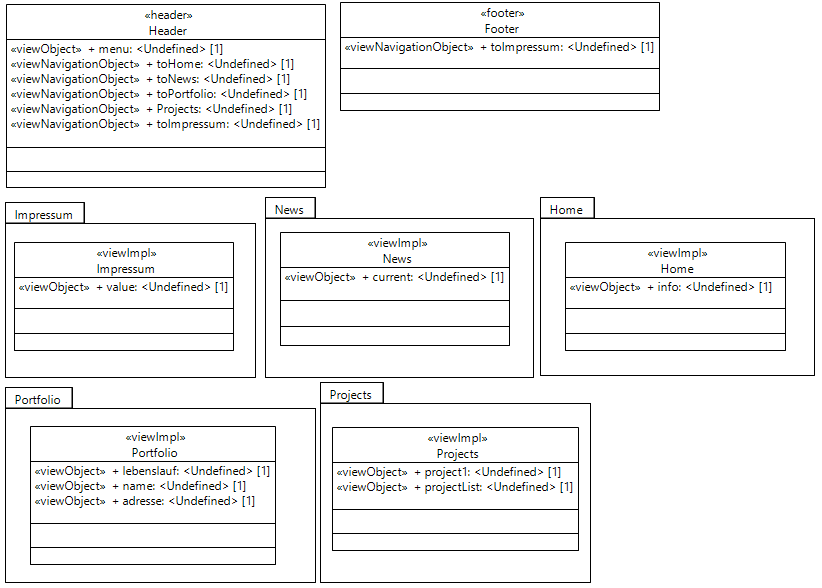
\includegraphics[width=0.8\textwidth]{./img/Model2.png}
\caption{Verwendetes Modell}\label{Fig:ergModell}
\end{center}
\end{figure}

Durch die extra eingebauten Pakete erweitert sich die Grundstruktur des
Projektes, in Abbildung \ref{Fig:packegeModel} ist auf der linken Seite die
komplette Packetstruktur des Projektes zu sehen. Hier ist zu erkennen, dass
für die fünf Seiten separate Pakete existieren. Jedoch für den Header und den
Footer keine zusätzlichen Pakete angelegt worden sind. Auf der rechten Seite in
Abbildung \ref{Fig:packegeModel}, wird der Inhalt einiger der Pakete näher
gezeigt. Hier ist zu erkennen, dass die beiden \texttt{ViewImpl}, die nicht in
Paketen liegen, direkt in dem \texttt{view} Paket liegen. Zusätzlich sind die
Klassen \texttt{Activity}, \texttt{Place}, \texttt{View} und die
\texttt{.ui.xml} Datei in dem Paket zu sehen. Am Beispiel der
\texttt{Home}-Seite ist gezeigt, dass die hierfür generierten Klassen und
Dateien in einem separaten Paket von \texttt{view}, nämlich in \texttt{home}
liegen.

\begin{figure}[htbp]
\begin{center}
\raisebox{3.2cm}{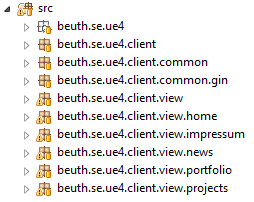
\includegraphics[width=0.4\textwidth]{./img/Packages.png}}
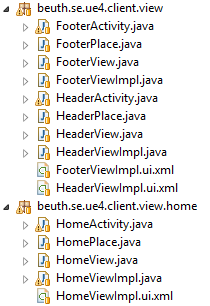
\includegraphics[width=0.4\textwidth]{./img/PackagesExample.png}
\caption{Generierte Paketstruktur, links gesamte
Paketstruktur im Überblick; rechts Beispiel für das
Strukturieren im Modell, mit zusätzlichen Paketen}\label{Fig:packegeModel}
\end{center}
\end{figure}
 
In diesem Beispiel soll die \texttt{home} Seite die Startseite für die
Webanwendung darstellen. Aus diesem Grund wurde entsprechend in der
\texttt{AppEntryPoint}- und der \texttt{ProductionGinModule}-Klasse die
jeweilige Klasse für die StartView angegeben. (Listing \ref{lst:appEntryPoint}
und \ref{lst:ProductionGinModule}) 
\lstset{language=gwt}
\begin{lstlisting}[caption={Änderung an der \texttt{AppEntryPoint}-Klasse zur
Bestimmung der Startseite}, label={lst:appEntryPoint}] 
[..]
  historyHandler.register(injector.getPlaceController(), eventBus,
      new HomePlace());
[..]
\end{lstlisting}
\lstset{language=gwt}
\begin{lstlisting}[caption={Änderung an der \texttt{ProductionGinModule}-Klasse
zur Bestimmung der Startseite}, label={lst:ProductionGinModule}] 
[..]
  bind(HomeView.class);
[..]
\end{lstlisting}

Zusätzlich wurde an einigen Stellen der Inhalt der Seiten erweitert. Dies ist
einerseits dadurch möglich, dass innerhalb der \texttt{ViewImpl} Klasse
zusätzlicher Inhalt eingefügt werden kann (Listing \ref{lst:conntentJava}), aber
anderseits innerhalb der \texttt{.ui.xml}-Datei (Listing \ref{lst:conntentUI}).

\lstset{language=gwt}
\begin{lstlisting}[caption={Einfügen von Inhalten auf einer Seite durch
Veränderungen am Java-Code},
label={lst:conntentJava}] 
[..] 
  HTML html = new HTML("<div><h1>Brandhei&szlig;e News</h1>"
	+"Lorem ipsum [..] amet."
	+"<div/>");
  content.add(html);
[..]
\end{lstlisting}
\lstset{language=gwt}
\begin{lstlisting}[caption={Einfügen von Inhalten auf einer Seite durch
Veränderungen am \texttt{ui.xml}-Datei},
label={lst:conntentUI}] 
[..] 
 <g:FlowPanel>
	<!-- InteractionElements -->
	<!-- Start of user code Home 
	     Start protectetRegion -->
			<g:Label text=" Lorem [..] facilisi. "/>
			[..]		
	<!-- End of user code -->
	</g:FlowPanel>
[..]
\end{lstlisting}

Dieses sind nur zwei Arten wie die Anwendung weiter bearbeitet werden kann,
nachdem der Quellecode aus dem M1 Modell generiert worden ist. Zum Einen
unterstützen der Generator und das Profil derzeit nicht alle von GWT
bereitgestellten UI Elemente, sodass diese nachträglich eingefügt werden
müssen. Da diverse UI Editoren existieren, welche das Erzeugen einer
Benutzeroberfläche grafisch unterstützen, wurde sich in dieser Arbeit bewusst
gegen das Erzeugen einer Webanwendung, die vollständig designt worden ist,
entschieden. 
